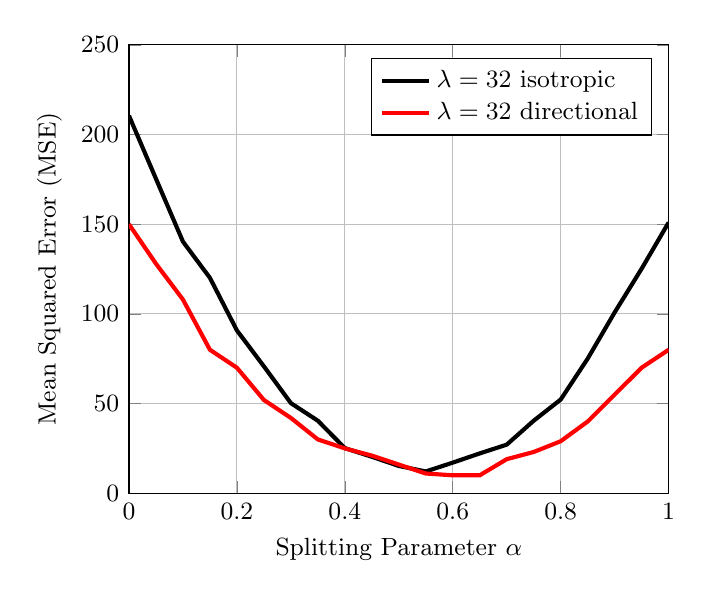
\begin{tikzpicture}
\begin{axis}[
font=\small,
xlabel= {Splitting Parameter $\alpha$},
ylabel= {Mean Squared Error (MSE)},
xmin = 0, xmax = 1,
ymin = 0, ymax = 250,
xmajorgrids,
ymajorgrids,
legend entries={$\lambda=32$ isotropic,$\lambda=32$ directional},
legend style={legend pos=north east,nodes=right}]

% Method: Bayes,
% Area Type = inscribed,
% Antenna Type = omnidirectional,
% Noise = 2,
% Trials = 50000,
% Total rate = 16,
% alpha_step =0.025,
% A_t =36.0,
% A_o =64.0,
% BMSE

\addplot [
color=black,
line width=1.5pt,
solid,
]
coordinates{
(0.0, 210.522)
(0.05, 175.363)
(0.1, 140.311)
(0.15, 120.097)
(0.2, 90.786)
(0.25, 70.768)
(0.3, 50.245)
(0.35, 40.432)
(0.4, 25.156)
(0.45, 20.332)
(0.5, 15.221)
(0.55, 12.140)
(0.6, 17.065)
(0.65, 22.211)
(0.7, 27.097)
(0.75, 40.456)
(0.8, 52.245)
(0.85, 75.064)
(0.9, 100.852)
(0.95, 125.219)
(1.0, 150.987)
};

% Method: Bayes,
% Area Type = inscribed,
% Antenna Type = directional,
% Noise = 2,
% Trials = 50000,
% Total rate = 16,
% alpha_step =0.025,
% A_t =36.0,
% A_o =64.0,
% BMSE


\addplot [
color=red,
line width=1.5pt,
solid,
]
coordinates{
	(0.0, 150)
	(0.05, 128)
	(0.1, 108)
	(0.15, 80)
	(0.2, 70)
	(0.25, 52)
	(0.3, 42)
	(0.35, 30)
	(0.4, 25)
	(0.45, 21)
	(0.5, 16)
	(0.55, 11)
	(0.6, 10)
	(0.65, 10)
	(0.7, 19)
	(0.75, 23)
	(0.8, 29)
	(0.85, 40)
	(0.9, 55)
	(0.95, 70)
	(1.0, 80)
};

\end{axis}

\end{tikzpicture}

